\documentclass[references.tex]{subfiles}
\begin{document}


\section{\citep{AndCri2011}}
\subsection{Summary}

This paper simplifies the ``enormous list of existing methods'' of 
analysing $\beta$ diversity, together with its multiple meanings. It 
concludes with a case study on Indonesean coral 
in order to to navigate multiple meanings of $\beta$ diversity.

Two types:
\begin{itemize}
    \item directional turnover along a gradient
    \item non-directional variation
\end{itemize}


\subsection{Questions and Thoughts}
\noindent
What exactly is \textbeta{} diversity?
\begin{itemize}
    \item variation in the identities of species among sites
    \item provides a direct link between biodiversity at local scales 
          ($\alpha$ diversity)
    \item and the broader regional species pool ($\gamma$ diversity)
\end{itemize}

\noindent
classes of \textbeta{} diversity:
\begin{itemize}
    \item classical metrics, calculated directly from $\gamma$ and $\alpha$ diversity
    \item multivariate measures, based on pairwise resemblances among sample units
\end{itemize}
\subsection{How this relates to my research}
\subsection{Notes}
\begin{itemize}
    \item \gls{bdiversity} 
    \begin{itemize}
        \item is composed of $\alpha$ (local) and $\gamma$ (regional) 
        diversity (not clear if components should be additive or multiplicative)
        \item used by many ecologists to describe relative abundance, 
        as well as taxonomic, phylogenetic, and functional relationships
        among species
    \end{itemize}
    \item statistical approaches to analysing $\beta$ diversity
\end{itemize}

Existing frameworks for $\beta$ diversity
\begin{itemize}
    \item \citep{JurRet2009}
    \begin{itemize}
        \item inventory
        \item differentiation
        \item proportional
    \end{itemize}
\end{itemize}

Types of $\beta$ diversity
\begin{itemize}
    \item \citep{Vel2001}
    \begin{itemize}
        \item turnover
        \item variation in community structure
   \end{itemize}
\end{itemize}

\begin{figure*}[h!]
    \centering
    \begin{tabular}{c}
    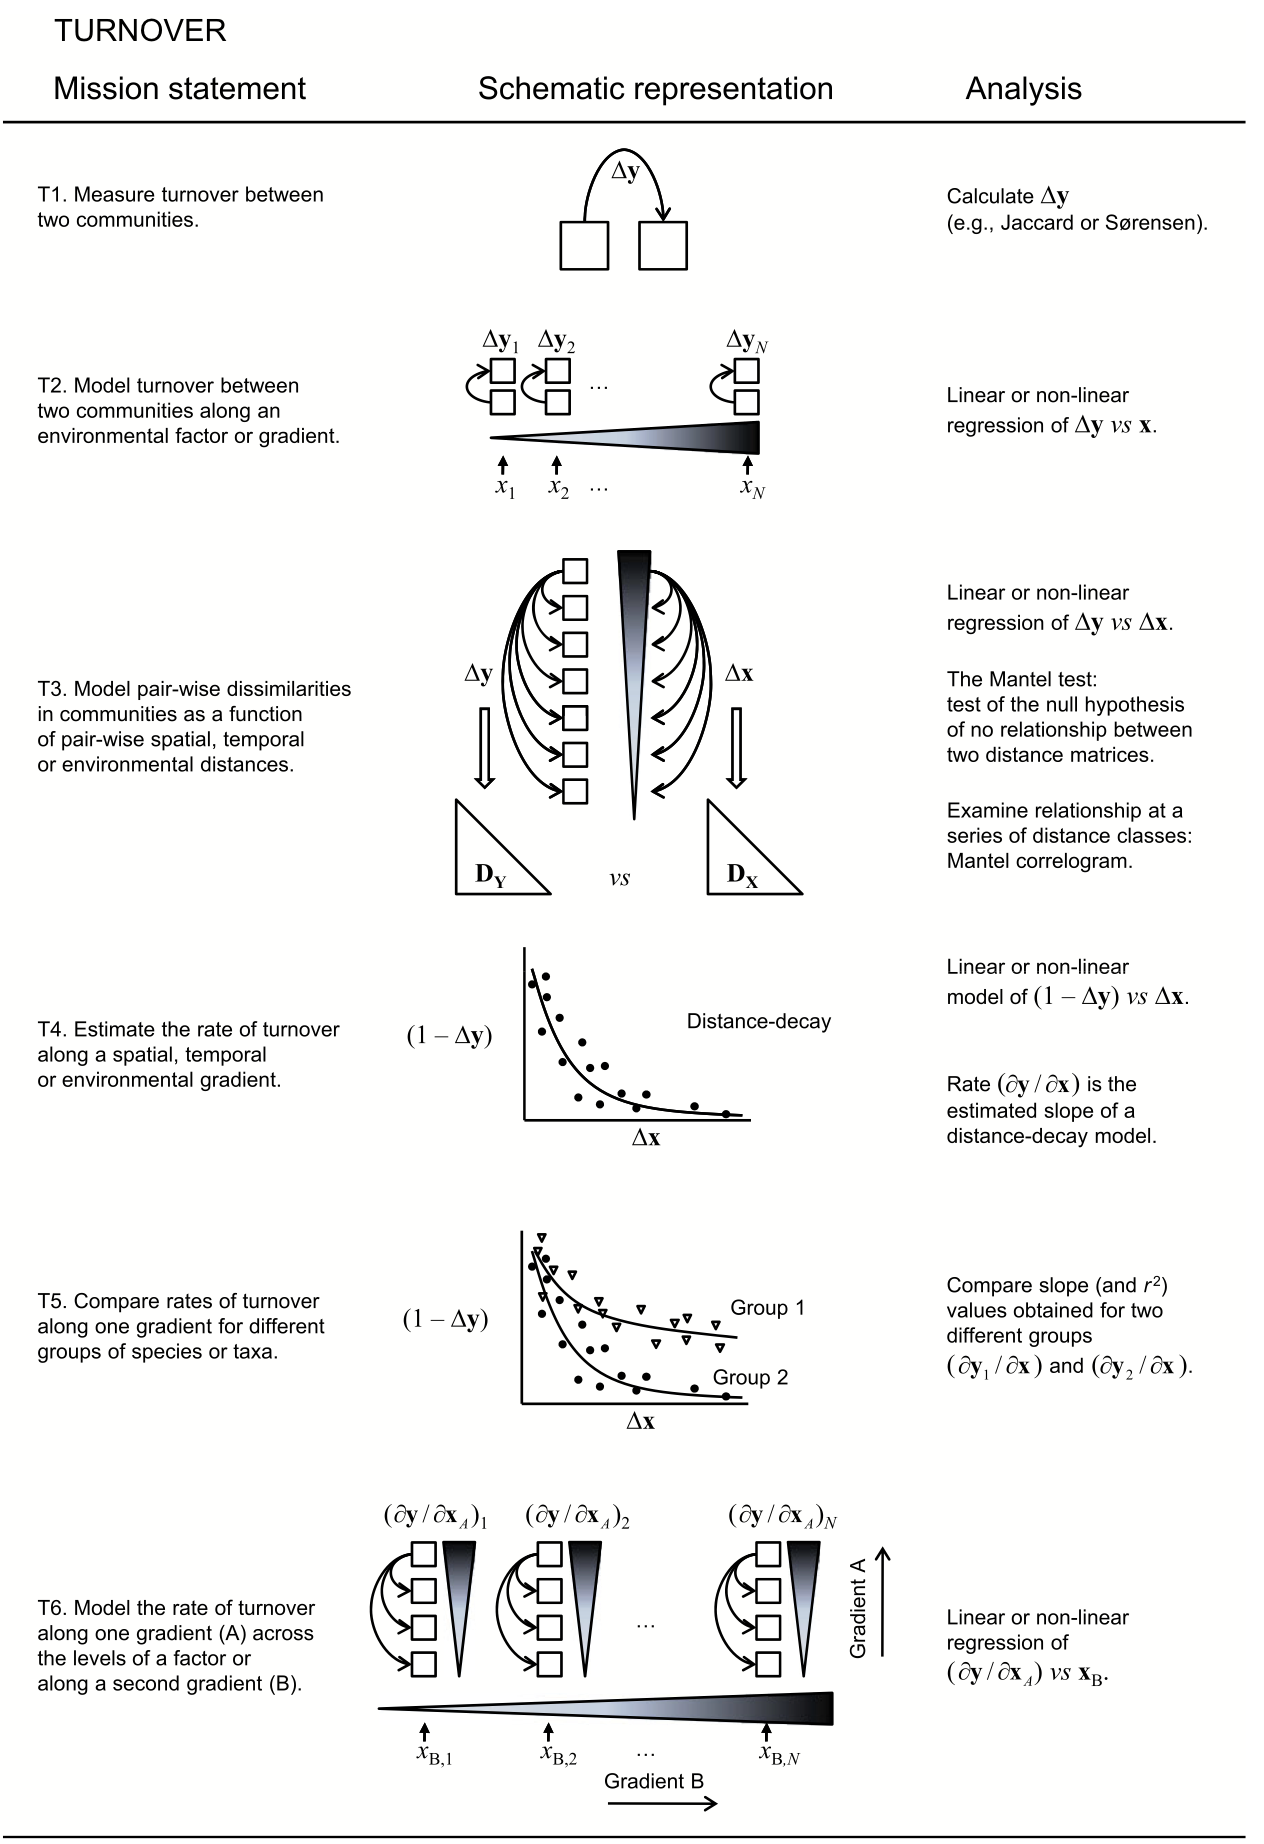
\includegraphics[scale=0.65]{images/figures/AndCri2011/fig3.png}
    \\\hline
    \end{tabular}
    \caption{
        figure 3 from \citep{AndCri2011}: schematic representation and appropriate analyses of ecological $\beta$ diversity for each of a series of mission statements with a focus on \textbf{turnover} along one or more spatial, temporal, or environmental gradients
    }
\end{figure*}


\begin{figure*}[h!]
    \centering
    \begin{tabular}{c}
    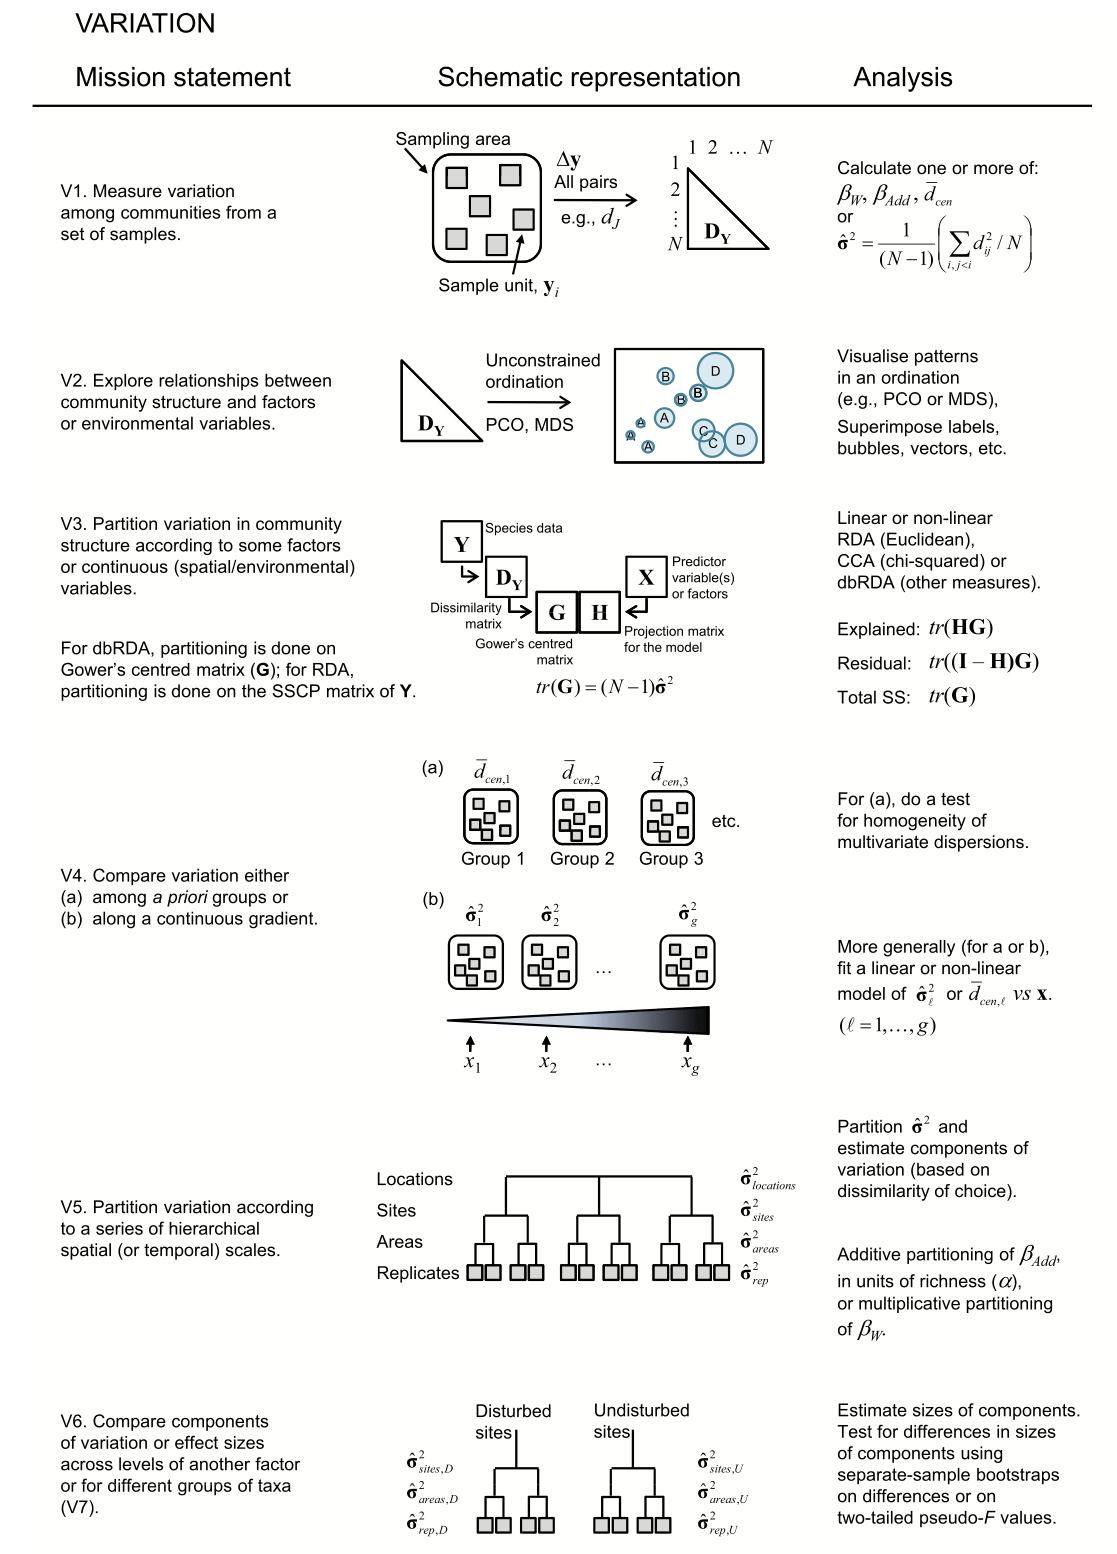
\includegraphics[scale=0.65]{images/figures/AndCri2011/fig4.png}
    \\\hline
    \end{tabular}
    \caption{
        figure 4 from \citep{AndCri2011}: schematic representation and appropriate analyses of ecological $\beta$ diversity for each of a series of mission statements with a focus on \textbf{variation} among sample units
    }
\end{figure*}



\bib{}
\end{document}